\section{ИССЛЕДОВАНИЕ РАБОТЫ ЦИФРОВОГО КОМПАРАТОРА}

\begin{figure}[H]
	\centering
	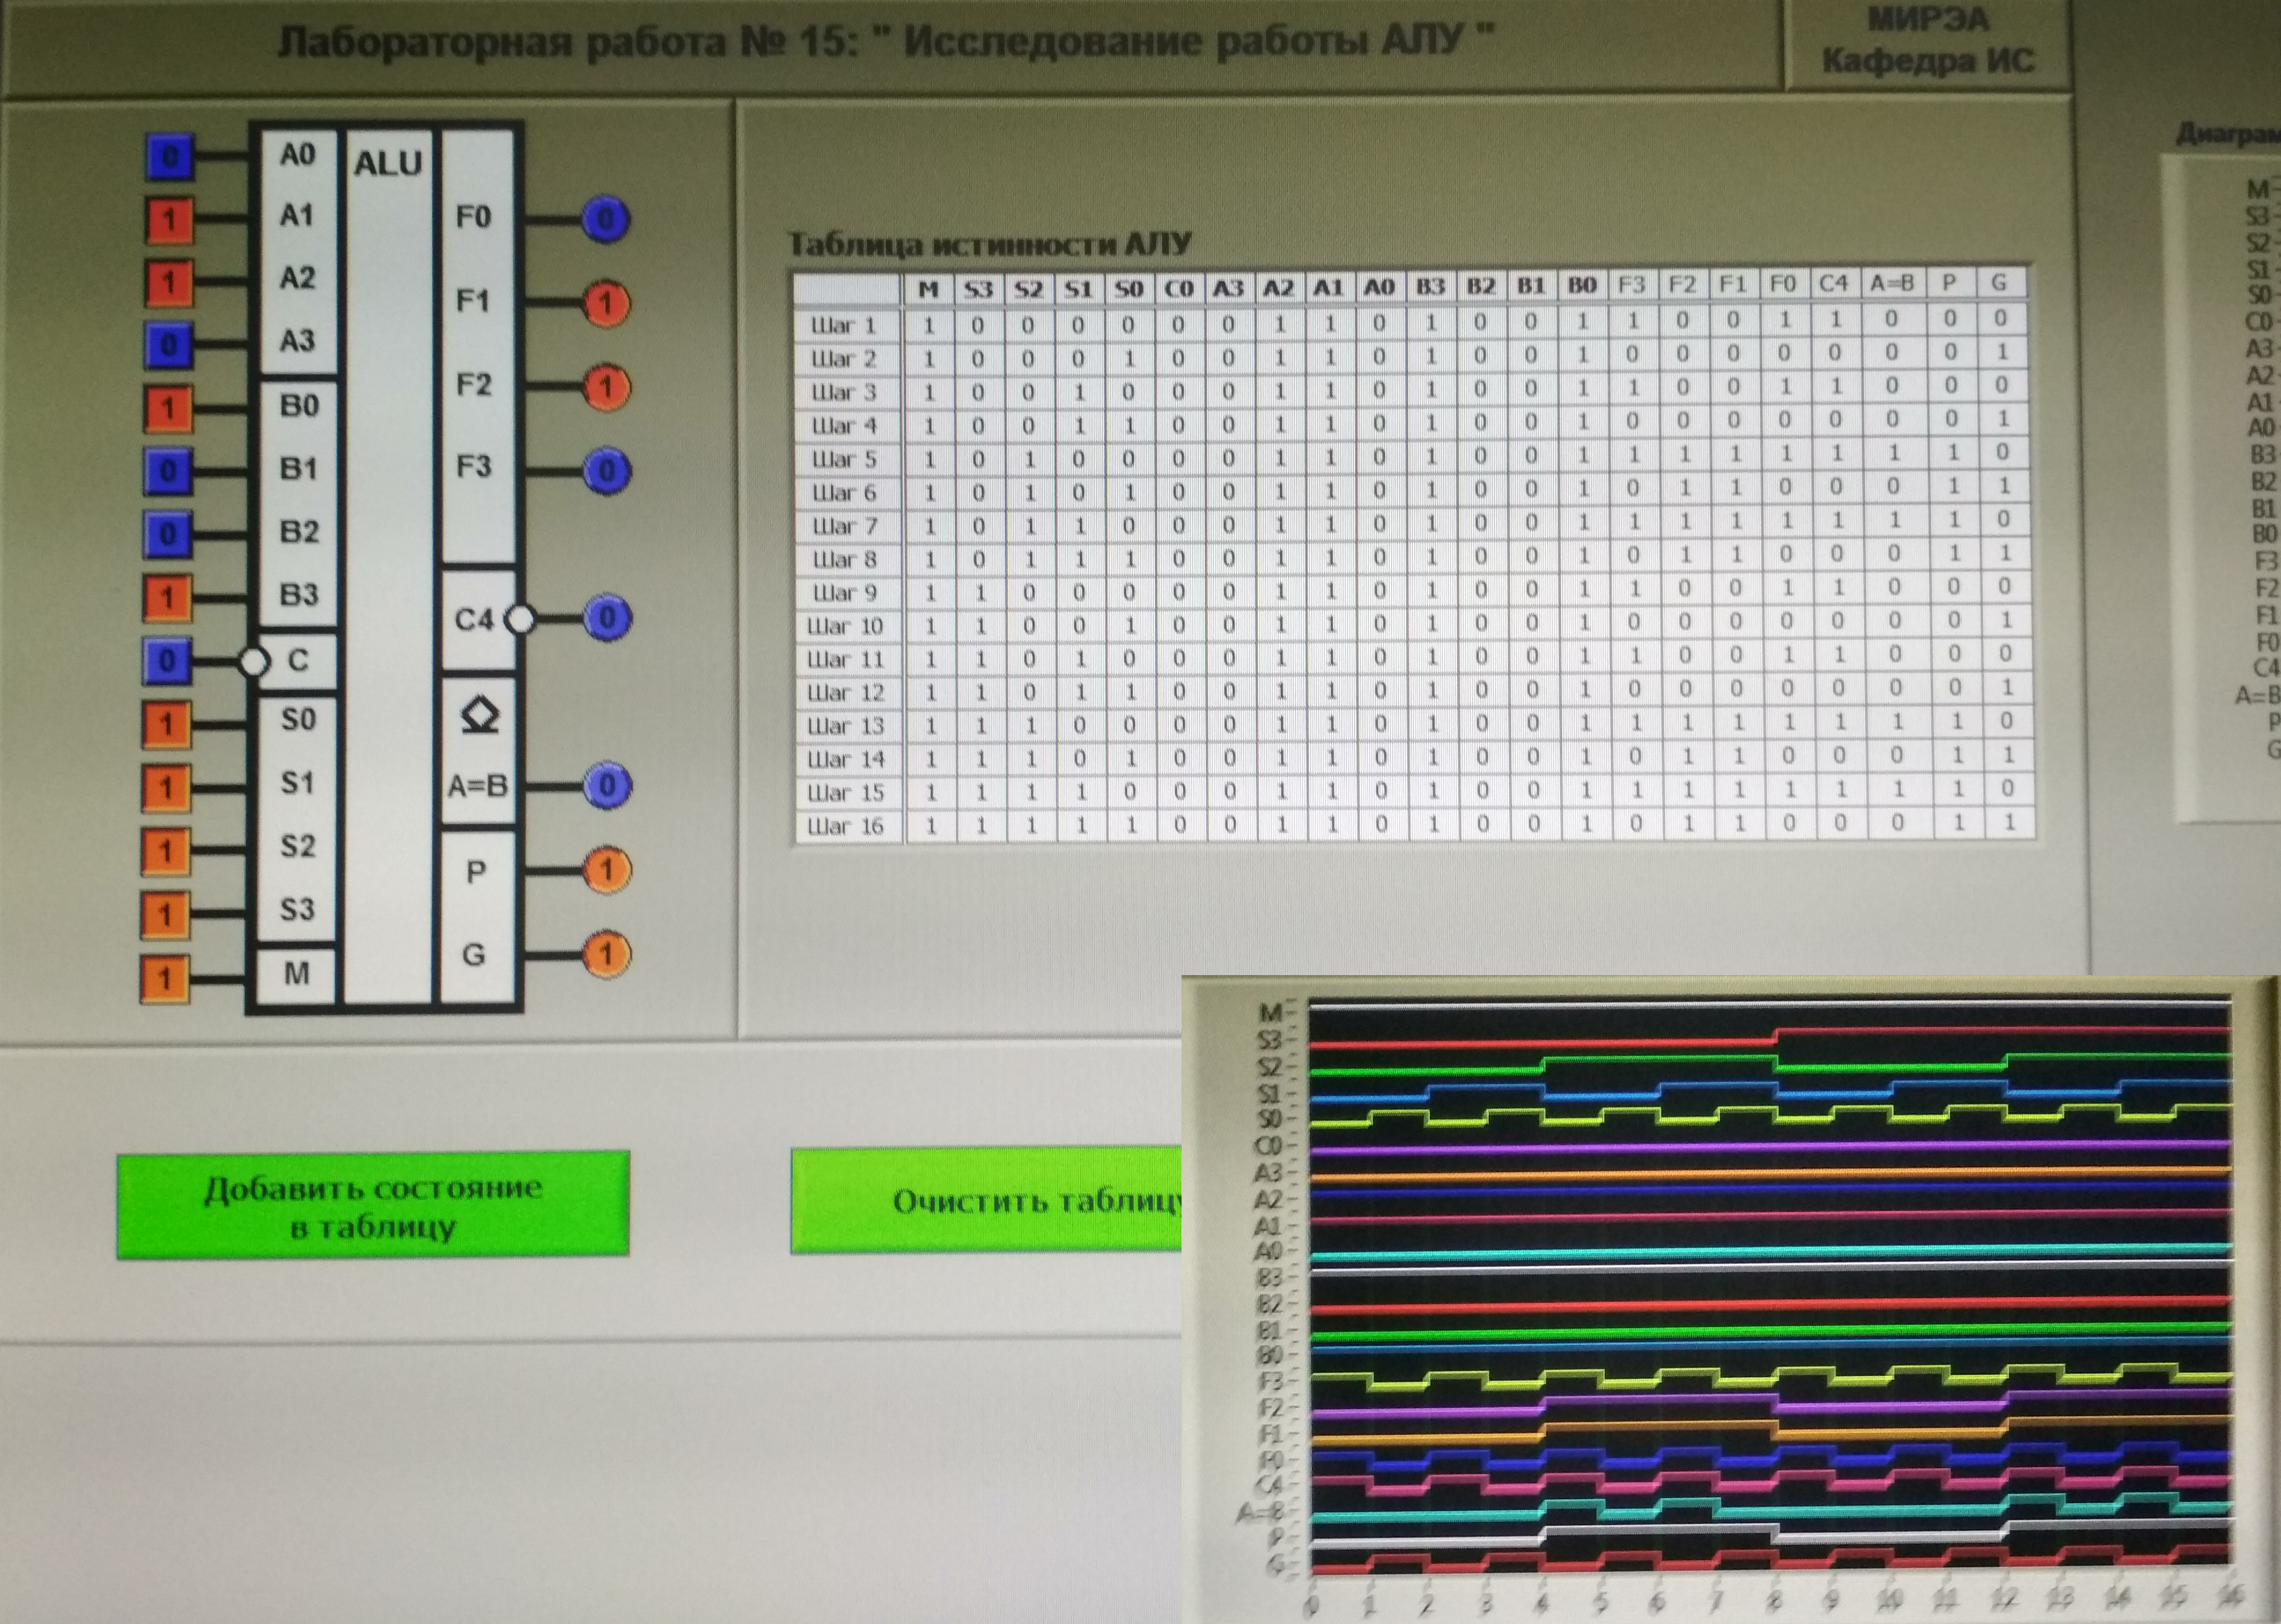
\includegraphics[width=0.95\linewidth]{imgs/6/1}
	\caption{Результат работы компаратора}
	\label{fig:6_}
\end{figure}

Для обработки пятиразрядного сигнала необходимо взять два компаратора и передать выход первого на входы управления второго, а на входы значений подать соответствующие пары. 
Оставшиеся входы должны иметь одинаковый уровень, поэтому их можно оставить как есть.

Элемент CD74HCT85 - High-Speed CMOS

Характеристики:

\begin{figure}[H]
	\centering
	\includegraphics[width=0.95\linewidth]{imgs/6/ti1}
	\caption{Электрические парамеры}
	\label{fig:6_ti1}
\end{figure}

\begin{figure}[H]
	\centering
	\includegraphics[width=0.95\linewidth]{imgs/6/ti2}
	\caption{Электрические парамеры}
	\label{fig:6_ti2}
\end{figure}

\begin{figure}[H]
	\centering
	\includegraphics[width=0.95\linewidth]{imgs/6/ti3}
	\caption{Параметры переключения}
	\label{fig:6_ti3}
\end{figure}


\begin{figure}[H]
	\centering
	\includegraphics[width=0.95\linewidth]{imgs/6/ti4}
	\caption{Параметры переключения}
	\label{fig:6_ti4}
\end{figure}
